% Name: Colormap with a colorbar
% Description: The electric potential of a dipole in the plane, colored on a diverging colormap whose colorbar gives the values, with the two charges marked.
% Tags: colormap, colorbar, density plot, electric potential

\usepackage{pgfplots}
\pgfplotsset{compat=1.18}

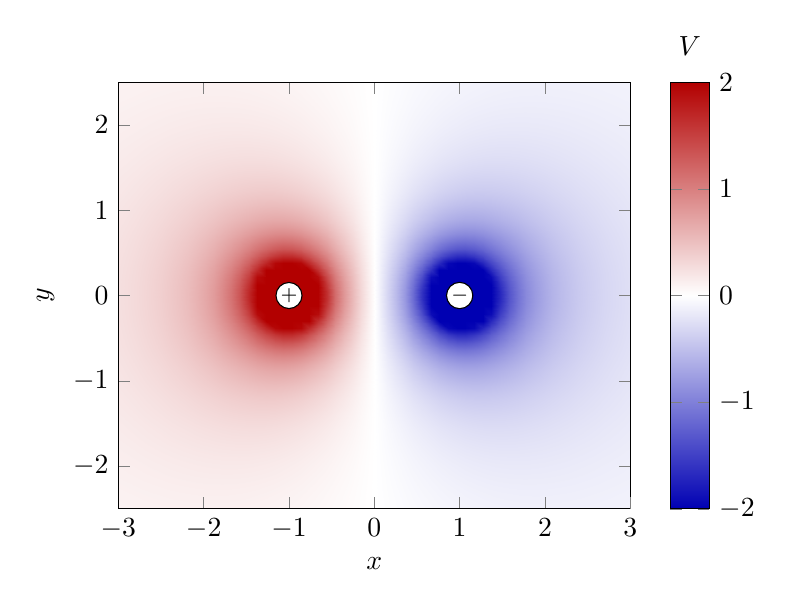
\begin{tikzpicture}
  \begin{axis}[
    width=8.5cm, height=7cm, view={0}{90}, axis equal image, enlargelimits=false,
    xlabel=$x$, ylabel=$y$, colorbar,
    colormap={diverging}{color=(blue!70!black) color=(white) color=(red!70!black)},
    point meta min=-2, point meta max=2,
    colorbar style={title={$V$}, ytick={-2,-1,0,1,2}},
  ]
    % Charges +1 at (-1, 0) and -1 at (1, 0); 60 samples keep the grid off the charges themselves.
    \addplot3[surf, shader=interp, domain=-3:3, domain y=-2.5:2.5, samples=60]
      {1/sqrt((x+1)^2 + y^2) - 1/sqrt((x-1)^2 + y^2)};
    \node[circle, fill=white, draw, inner sep=0.5pt, font=\scriptsize] at (axis cs:-1,0,3) {$+$};
    \node[circle, fill=white, draw, inner sep=0.5pt, font=\scriptsize] at (axis cs:1,0,3) {$-$};
  \end{axis}
\end{tikzpicture}
